
%% Template for ENG 401 reports
%% by Robin Turner
%% Adapted from the IEEE peer review template

%
% note that the "draftcls" or "draftclsnofoot", not "draft", option
% should be used if it is desired that the figures are to be displayed in
% draft mode.

\documentclass[peerreview]{IEEEtran}
\usepackage{url} % Provides better formatting of URLs.
\usepackage[utf8]{inputenc} % Allows Turkish characters.
\usepackage{booktabs} % Allows the use of \toprule, \midrule and \bottomrule in tables for horizontal lines
\usepackage{graphicx}

\usepackage[backend=biber, style=alphabetic, isbn=true, doi=true]{biblatex}
\usepackage{csquotes}
\hyphenation{op-tical net-works semi-conduc-tor} % Corrects some bad hyphenation

\addbibresource{literatur.bib}


\usepackage{listings}
\usepackage{xcolor}

\definecolor{codegray}{gray}{0.9}
\definecolor{commentgreen}{rgb}{0,0.6,0}
\definecolor{keywordblue}{rgb}{0.2,0.2,0.8}

\lstdefinestyle{javastyle}{
    backgroundcolor=\color{white},
    commentstyle=\color{commentgreen}\itshape,
    keywordstyle=\color{keywordblue}\bfseries,
    numberstyle=\tiny\color{gray},
    stringstyle=\color{red},
    basicstyle=\ttfamily\small,
    breaklines=true,
    captionpos=b,
    keepspaces=true,
    numbers=left,
    numbersep=5pt,
    showspaces=false,
    showstringspaces=false,
    showtabs=false,
    tabsize=2,
    language=Java
}


\begin{document}
%\begin{titlepage}
% paper title
% can use linebreaks \\ within to get better formatting as desired
\title{Runtime Analysis of Shellsort \\with Emphasis on Worst-Case Complexity}


% author names and affiliations

\author{Thorsten Suckow-Homberg \\
Master's Student M.C.Sc.\\
Trier University of Applied Science
}
\date{21.05.2025}

% make the title area
\maketitle
\tableofcontents
\listoffigures
\listoftables
%\end{titlepage}

\IEEEpeerreviewmaketitle



\begin{abstract}
    This report investigates the time complexity of the Shellsort algorithm , based on both empirical measurements and formal analysis, with a particular focus on key arrangements that lead to worst-case behavior.

    Using a classic increment sequence of the form $h_t = \lfloor \frac{n}{2^t} \rfloor$, we analyze the number of element comparisons and swaps during the sorting process. Empirical data suggests a runtime between $O(n\ \log\ n)$ and $O(n^{1.3})$, while worst case-conditions yield a theoretical bound of $O(n^2)$. The report includes step-by-step code analysis and provides visual illustrations of best and worst-case inputs.


\end{abstract}
\section{Introduction}

\textbf{Shellsort}, introduced by \textit{Donald Shell} in 1959 (\cite[]{She59}), is a generalization of insertion sort\footnote{
see \cite[250]{SW11} for a brief introduction on insertion sort
} that improves performance by initially sorting elements far apart, yielding optimized arranged sequences of keys for subsequent passes.
The algorithm uses a sequence of decrementing gaps, comparing elements separated by a distance of $h_t$.\footnote{
hence, Shellsort is also referred to as ``diminishing increment sort`` (\cite[88]{OW17b})
}.
The general idea is to use \blockquote[{\cite[48]{CL22}}]{
    insertion sort on periodic subarrays of the input
    to produce a faster sorting algorithm.
}

\subsection{Algorithm Description and Notation}
We use the Shellsort implementation shown in Listing~\ref{lst:shell}.
In the following, we provide a brief description of the algorithm, mostly based on~\cite[84]{Knu97b}.
Throughout this document, the binary logarithm $\log_2$ is abbreviated as $\lg$.


Given an input of size $n$, the implementation based on a halving sequence of the form $h_t = \lfloor \frac{n}{2^t} \rfloor$ performs approximately $\lg\ n$ passes.
For this, an \textbf{increment sequence} $h$ is defined that determines the distance between two elements compared during sorting.
For instance, for $n = 16$, we choose $t=\lg n = 4$, resulting in the sequence $(8, 4, 2, 1)$ with

\[
    h_{3} = \lfloor\frac{16}{2^1}\rfloor = 8, h_{2} = \lfloor\frac{16}{2^2}\rfloor = 4, \ldots , h_{0} = \lfloor\frac{16}{2^4}\rfloor = 1
\]

such that

\[
    h_i = \lfloor {\frac{n}{2^{t-i}}} \rfloor
\]

for $0 \leq i \leq t - 1$.\\

In the first pass, the algorithm compares and sorts elements that are $h_{3} = \frac{16}{2^{4-3}} = 8$ positions apart, while the final pass processes keys $h_0 = \frac{16}{2^{4-0}} = 1$ positions apart, effectively performing \textit{insertion sort}.\\

To further illustrate runtime behavior, we define counting variables $c_1, c_2, c_3, c_4$ corresponding to lines 2, 5, 7 and 9 of the implementation.

\vspace{4mm}
\begin{lstlisting}[style=javastyle, caption={Shellsort implementation using halving sequences. }, label=lst:shell]
while (incr > 0) {
    c1++;
    for (i = incr; i < n.length; i++) {
        j = i - incr;
        c2++;
        while (j >= 0) {
            c3++;
            if (n[j] > n[j + incr]) {
                c4++;
                swap(n, j, j + incr);
                j = j - incr;
            } else {
                break;
            }
        }
    }
    incr = incr / 2;
}
\end{lstlisting}
\vspace{4mm}


\subsection{Role of the Increment Sequence Regarding Complexity}

As demonstrated by \textit{Knuth} in~\cite[91]{Knu97b}, the performance of Shellsort heavily  depends on the chosen increment sequence $h$: In particular, an upper bound of $O(n^{\frac{3}{2}})$ can be achieved\footnote{
\textit{Knuth} refers to the work of \textit{Papernov and Stasevich} \cite{PS65} in this context.
}, if the sequence satisfies

\[
    h_s = 2^{s+1} - 1, 0 \leq s < t = \lfloor{\lg n} \rfloor
\]

In our case, where a trivial halving sequence is used, we conservatively assume an upper bound of $O(n^2)$.

\section{Empirical Determination of Comparison Operations}

We empirically determine the number of comparisons between array elements for large, randomly generated arrays.
For Shellsort, we expect the runtime complexity to lie between $O(n\ \lg\ n)$ and $O(n^2)$.

To count the number of element comparisons, a counting variable $c_3$ can be employed, as illustrated in Listing~\ref{lst:shell}.
This variable increments each time an element comparison is performed.

Random arrays can be generated according to the method shown in Listing~\ref{lst:rand}, and the observed values of $c_3$ are recorded.
Since every comparison-based sorting algorithm belongs to the complexity class $\Omega(n\ \lg\ n)$, it is reasonable to assume that, on average, $c_3 \geq n\ \lg\ n$ holds (\cite[154]{OW17b}).\\

However, it should be noted that the function $n^{\frac{4}{3}} = n^{1.\overline{3}}$ grows faster than $n\ \lg\ n$ for input sizes $n \geq 982$ (see Figure~\ref{fig:lognplot}).

\begin{figure}[!h]
    \centering
    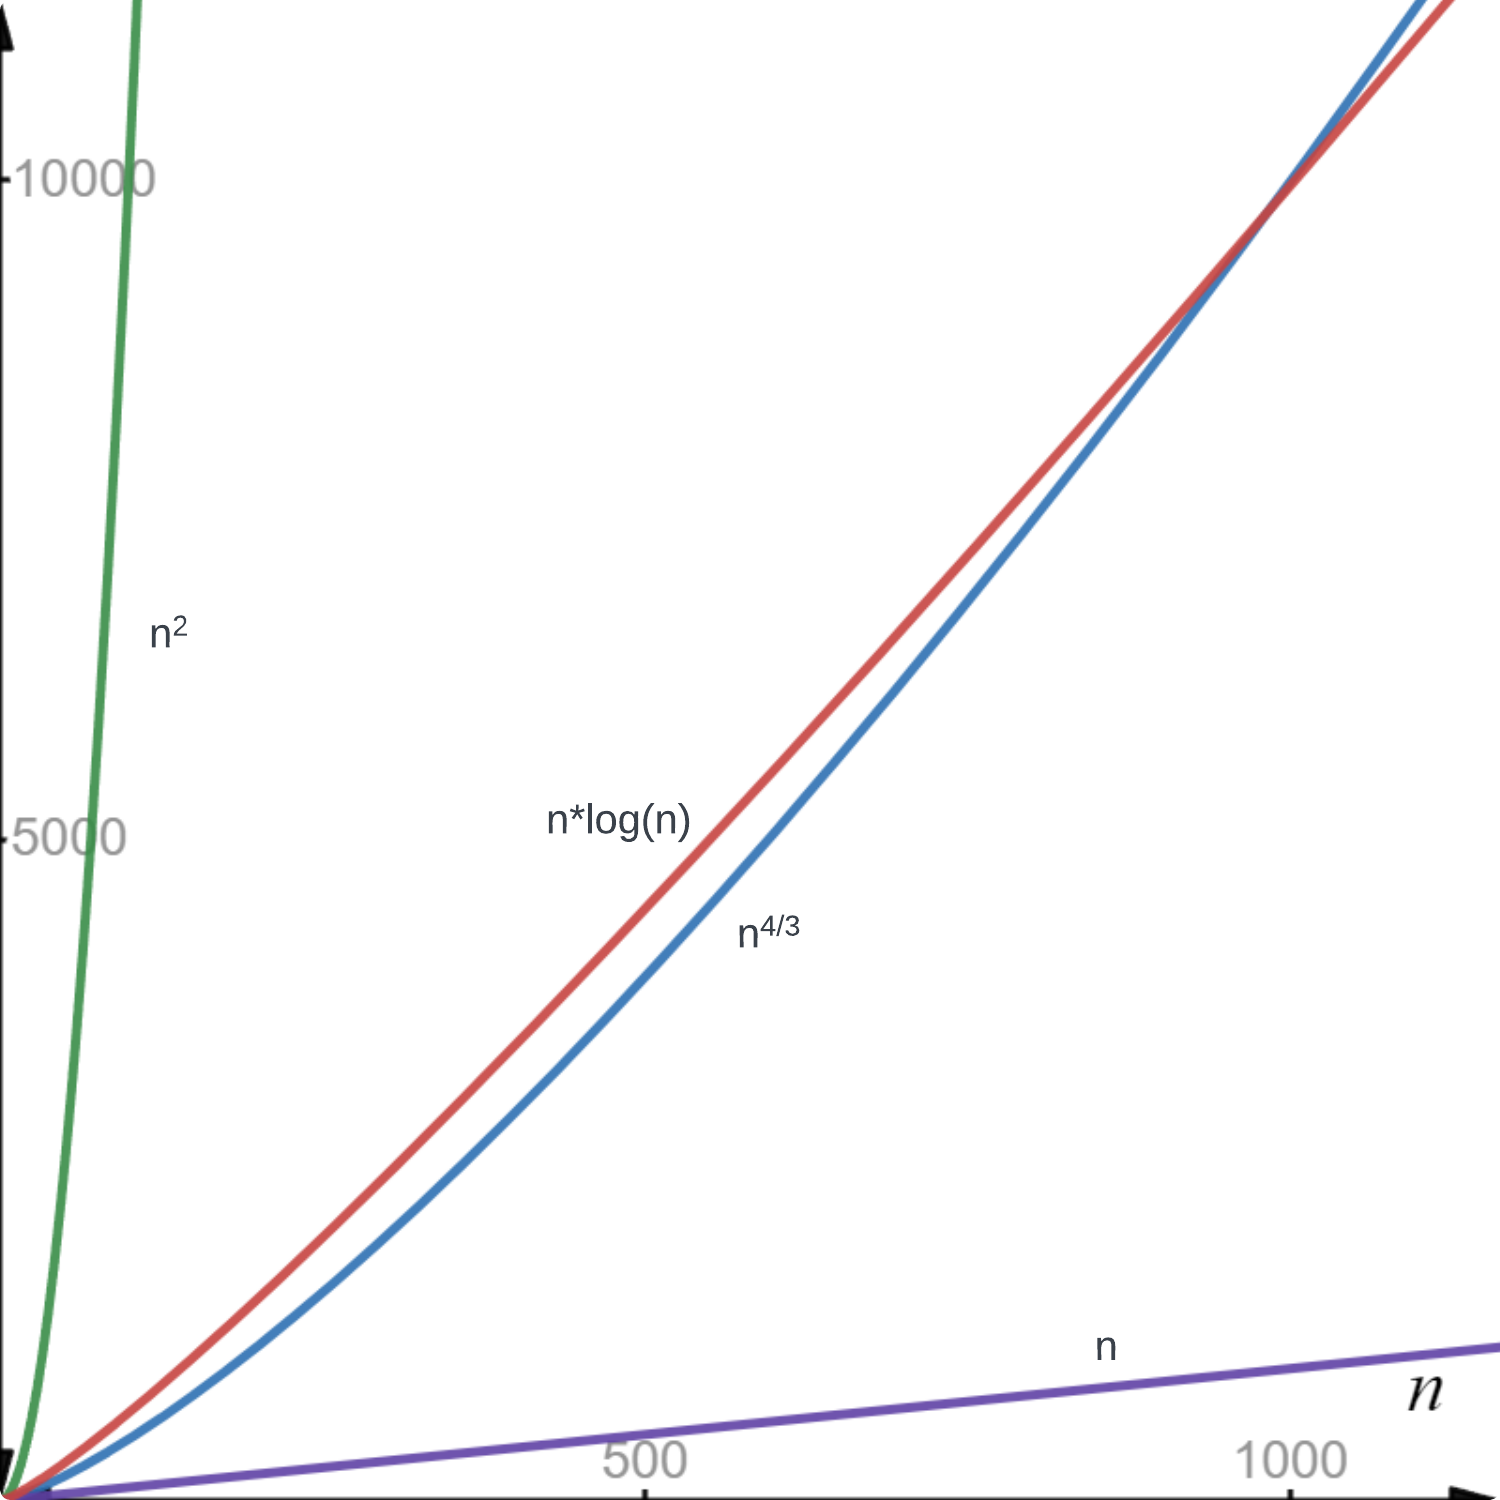
\includegraphics[width=0.8\columnwidth]{img/lognplot}
    \caption{For $n \geq 982$, $n^{\frac{4}{3}}$ grows faster than $n\ \lg\ n$.}
    \label{fig:lognplot}
\end{figure}


This behavior must be carefully considered when interpreting empirical results for smaller $n$.
Otherwise, one might incorrectly conclude that Shellsort achieves optimal runtime complexity of $O(n\ \lg\ n)$, disregarding the potential higher worst-case behavior.

\vspace{4mm}
\begin{lstlisting}[style=javastyle, caption={Code for Shellsort-testing large randomized arrays.}, label=lst:rand]
int epochs = 100;
while(epochs-- >= 0) {
    int[] tests = new int[]{
        2_000_000 /*, 4_000_000, ...*/
    };
    Random r = new Random();
    for (int i = 0; i < tests.length; i++) {
        int l = tests[i];
        int[] arr = new int[l];

        for (int j = l; j > 0; j--) {
            arr[l - j] = r.nextInt(l + 1);
        }

        ShellSort.sort(
            Arrays.copyOfRange(
                arr, 0, arr.length));
    }
}
\end{lstlisting}
\vspace{4mm}

\subsection{Test Results}
With 100 epochs and array sizes up to $n = 2.000.000$, the test from Listing~\ref{lst:rand} yielded the following distribution of observed comparison counts $c_3$:

\begin{itemize}
    \item In 74 out of 100 cases, the measured $c_3$ satisfied $n^{\frac{4}{3}} < c_3 < n^2$.
    \item In 26 out of 100 cases, the measured $c_3$ lay between $n\ \lg\ n$ and $n^{\frac{4}{3}}$, i.e., $n\ \lg\ n < c_3 < n^{\frac{4}{3}}$.
\end{itemize}

These results support the hypothesis that Shellsort often exhibits sub-quadratic runtime behavior, but does not consistently remain within the $O(n\ \lg\ n)$ bound.
Due to the lower bound $\Omega(n\ \lg\ n)$ for all comparison-based sorting algorithms, we are particularly interested in the empirical comparison counts $c_3$ within the following intervals:

\begin{itemize}
    \item $n \lg\ n \leq c_3 < n^{\frac{4}{3}}$
    \item $n^{\frac{4}{3}} \leq c_3 \leq n^2$
\end{itemize}

Test execution with large values of $n$ indicates that the number of comparisons $c_3$ falls either below $n^{\frac{4}{3}}$ or between $n^{\frac{4}{3}}$ and $n^2$, depending on the input.
This aligns with early empirical findings by \textit{Donald Shell}, who observed:

\blockquote[{\cite[31]{She59}}]{
It appears that the time required to sort $n$ elements is proportional to $n^{1.226}$.
}








\section{Problem Definition}
This will be a revised version of the problem definition in your proposal.


% An example of a floating figure using the graphicx package.
% Note that \label must occur AFTER (or within) \caption.
% For figures, \caption should occur after the \includegraphics.
% Note that IEEEtran v1.7 and later has special internal code that
% is designed to preserve the operation of \label within \caption
% even when the captionsoff option is in effect. However, because
% of issues like this, it may be the safest practice to put all your
% \label just after \caption rather than within \caption{}.
%
% Reminder: the "draftcls" or "draftclsnofoot", not "draft", class
% option should be used if it is desired that the figures are to be
% displayed while in draft mode.
%
\begin{figure}[!h]
\centering
\includegraphics[width=0.8\columnwidth]{trilece}
\caption{Simulation Results}
\label{fig_sim}
\end{figure}

% Note that IEEE typically puts floats only at the top, even when this
% results in a large percentage of a column being occupied by floats.

\section{Proposed Solutions}
This may be a modified version of your proposal depending on previously carried out research or any feedback received.
\subsection{Your first solution}
Describe your first solution here.
\subsection{Your second solution}
Describe your second solution here.
\subsection{Your third solution}
Describe your third solution here.
\subsubsection{Subsubsection Heading Here}
Use the subsubsection command with caution---you probably won't need it at, but I'm including it this an example.

\section{Criteria for Assessing Solutions} \label{sec:criteria}
This may be a modified version of your proposal depending on previously carried out research or any feedback received.



\section{Research Methodology}
The main difference between this section and the one in your report proposal is use of verb tense: there you suggested what you will do and here you will describe what you did. Be concise and precise when outlining how you researched your potential solutions.
Remember that your research should be guided by:
\begin{itemize}
\item Relevance to the context of application
\item Your assessment criteria
\item Practicality
\end{itemize}
So it may be worth commenting on your research methodology in light of the above (e.g., justifying a particular approach).

In this section, only describe how you collected data, and explain what you did to test your criteria.  \emph{Do not include your findings in this section.}

\section{Analysis and Interpretation}
 In this section you will mainly analyze your data in terms of your assessment criteria; e.g., do the data suggest that a particular solution is ``cost effective'' ``environmentally acceptable'', ``technically feasible'' or ``affordable''?

Be logical and selective when analyzing/interpreting your research data.  For example, if a proposed solution is proven to be far too expensive to realistically implement in your context, is there any value in discussing whether it is ``culturally viable'' or ``technically sustainable''? Perhaps in this case you can focus more attention on solutions that your research suggests are more valid.  Do not just throw huge quantities of raw data at your reader and leave them to interpret it. Present enough to transparently support any conclusions you draw and make sure that you offer justifications for your analysis.

Be honest and reflective while discussing your data. Your data might be too limited or unclear to interpret with accuracy---explain this, perhaps suggesting how this shortcoming could be addressed. Admitting the above will help you draw more honest and worthwhile conclusions.

Remember that research is an imperfect and ongoing process that should be open to question and verification. Therefore, unless convinced by the absolute strength of your evidence, you should be tentative in your language choice when interpreting/analyzing research results. Selectively use {\em hedging} (language which indicates a lack of certainty) to modify the tone of your analysis and any conclusions that result from this.

Here are some examples that show differing degrees of certainty:
\begin{itemize}
\item it appears that \ldots
\item it can be tentatively concluded that \ldots
\item it is almost certain that \ldots
\item perhaps the evidence indicates \ldots
\item this seems to point to the fact that \ldots
\item this could be interpreted as evidence of \ldots
\item without doubt its application would prove beneficial for \ldots
\end{itemize}

Finally, don’t introduce any new content (e.g., research methods or solutions) within this section---this will prove confusing for the reader. The reader should clearly understand that you are, based on specific criteria, interpreting the results of your research in order to test the viability of various solutions to remedy a particular problem. The sole function of this part of the report is to openly discuss your research findings in order to set up your conclusions/recommendations.


% Example of a table from http://www.latextemplates.com/template/professional-table
\begin{table} % Add the following just after the closing bracket on this line to specify a position for the table on the page: [h], [t], [b] or [p] - these mean: here, top, bottom and on a separate page, respectively
\centering % Centers the table on the page, comment out to left-justify
\begin{tabular}{l c c c c c} % The final bracket specifies the number of columns in the table along with left and right borders which are specified using vertical bars (|); each column can be left, right or center-justified using l, r or c. To specify a precise width, use p{width}, e.g. p{5cm}
\toprule % Top horizontal line
& \multicolumn{5}{c}{Growth Media} \\ % Amalgamating several columns into one cell is done using the \multicolumn command as seen on this line
\cmidrule(l){2-6} % Horizontal line spanning less than the full width of the table - you can add (r) or (l) just before the opening curly bracket to shorten the rule on the left or right side
Strain & 1 & 2 & 3 & 4 & 5\\ % Column names row
\midrule % In-table horizontal line
GDS1002 & 0.962 & 0.821 & 0.356 & 0.682 & 0.801\\ % Content row 1
NWN652 & 0.981 & 0.891 & 0.527 & 0.574 & 0.984\\ % Content row 2
PPD234 & 0.915 & 0.936 & 0.491 & 0.276 & 0.965\\ % Content row 3
JSB126 & 0.828 & 0.827 & 0.528 & 0.518 & 0.926\\ % Content row 4
JSB724 & 0.916 & 0.933 & 0.482 & 0.644 & 0.937\\ % Content row 5
\midrule % In-table horizontal line
\midrule % In-table horizontal line
Average Rate & 0.920 & 0.882 & 0.477 & 0.539 & 0.923\\ % Summary/total row
\bottomrule % Bottom horizontal line
\end{tabular}
\smallskip
\caption{Some impressive numbers} % Table caption, can be commented out if no caption is required
\label{tab:template} % A label for referencing this table elsewhere, references are used in text as \ref{label}
\end{table}
A reference to Table \ref{tab:template}.

\section{Conclusions and Recommendations}
Conclusion shows what knowledge comes out of the report. As you draw a conclusion, you need to explain it in terms of the preceding discussion. You are expected to repeat the most important ideas you have presented, without copying. Adding a table/chart summarizing the results of your findings might be helpful for the reader to clearly see the most optimum solution(s).

It is likely that you will briefly describe the comparative effectiveness and suitability of your proposed solutions. Your description will logically recycle language used in your assessing criteria (section \ref{sec:criteria}): ``Solution A proved to be the most cost effective of the alternatives'' or ``Solution B, though a viable option in other contexts, was shown to lack adaptability''.  Do not have detailed analysis or lengthy discussions in this section, as this should have been completed in section X.

As for recommendations, you need to explain what actions the report calls for. These recommendations should be honest, logical and practical. You may suggest that one, a combination, all or none of your proposed solutions should be implemented in order to address your specific problem. You could also urge others to research the issue further, propose a plan of action or simply admit that the problem is either insoluble or has a low priority in its present state.

The recommendations should be clearly connected to the results of the report, and they should be explicitly presented. Your audience should not have to guess at what you intend to say.




\appendices
\section{What Goes in the Appendices} \label{App:WhatGoes}
The appendix is for material that readers only need to know if they are studying the report in depth. Relevant charts, big tables of data, large maps, graphs, etc. that were part of the research, but would distract the flow of the report should be given in the Appendices.
\section{Formatting the Appendices} \label{App:Formatting}
Each appendix needs to be given a letter (A, B, C, etc.) and a title. \LaTeX will do the lettering automatically.






%\bibliographystyle{geralpha}			% Literaturverzeichnis
%\bibliography{literatur}     			% BibTeX-File literatur.bib
%\raggedright
\sloppy
\printbibliography
\fussy








\end{document}
